\chapter{Transonic Nozzle Flow Reconstruction}
\label{chap:Case_Study}

To evaluate the performance of the method, a case study was selected for the reconstruction of supersonic flow of hot air inside a nozzle. The availability of experimental data and a comprehensive apparatus description \citep{Back1965a} provided us with the necessary resources to validate the numerical methods used to generate training and test datasets. This case study also poses a challenging scenario for the surrogate model, involving the reconstruction of flow fields with discontinuous shock wave structures.

In this case study we perform a dimensiolaity reduction study to investigate the impact of the reduced basis dimension on the overall reconstruction strategy, the model accuracy was also evaluate in function of three diffent data set sizes and also with respect to the construction of the entry quantities in the low fidelity data matrix $\mathbf{x}$. We also performed neural network hyperparameter optimization and compared the results agains the Gaussian process method.

%To accurately predict this complex flow field, we can utilize the Reynolds-Averaged Navier-Stokes Equations. This simulation, which accounts for compressible and viscous effects, including shock formation in a 2D domain, for this reason this simulation as the \textit{high-fidelity} simulation. However, this simulation comes with its drawback in terms of computational cost. To mitigate this, we can obtain an approximate numerical solution using the quasi one-dimensional Euler equations, known as the \textit{low-fidelity} simulation, as it is a non-viscous model.


\section{The Nozzle Geometry}

The fluid behavior inside the nozzle is largely dependent not only on thermodynamic boundary conditions on its entrance and exits, but also on the geometric configuration of the walls. To made the surrogate model sentive to the geometric configuration the nozzle was constructed in parametrically in a CAD software (opensource FreeCAD), following the parameters of the $45^\circ-15^\circ$ nozzle described in \cite{Back1965a} and listed in Table \ref{tab:geom_params}.

\begin{table}[h]
    \centering
        \begin{tabular}{ r l r l }
            \hline
            \textbf{description}               & \textbf{parameter} & \textbf{value} & \textbf{units} \\ 
            \hline
            \hline
            \symbl{$L_i$}{Distante to $r_i$ center}
            {Distante to $r_i$ center}           & $L_{i}$         & 7.874   & mm \\
            \symbl{$L_{tht1}$}{Convergent $r_c$ tangency distance}
            {Convergent $r_c$ tangency distance} & $L_{tht1}$      & 55.880  & mm \\
            \symbl{$L_{tht2}$}{Divergent $r_c$ tangency distance}
            {Divergent $r_c$ tangency distance}  & $L_{tht2}$      & 68.148  & mm \\
            \symbl{$L_{th}$}{Length to throat}
            {Length to throat}                   & $L_{th}$        & 64.872  & mm \\
            \symbl{$L_{ti}$}{Length to $r_i$ tangency}
            {Length to $r_i$ tangency}           & $L_{ti}$        & 22.250  & mm \\
            \symbl{$L_{to}$}{Length to $r_o$ tangency}
            {Full length}                        & $L$             & 185.039 & mm \\
            \symbl{$r_{c}$}{Curvature radius at contraction}
            {Curvature radius at contraction}    & $r_{c}$         & 12.700  & mm \\
            \symbl{$r_{i}$}{Curvature radius at inlet}
            {Curvature radius at inlet}          & $r_{i}$         & 20.320  & mm \\
            \symbl{$r_{in}$}{Inlet radius}
            {Inlet radius}                       & $r_{in}$        & 63.500  & mm \\
            \symbl{$r_{th}$}{Throat radius}
            {Throat radius}                      & $r_{th}$        & 20.320  & mm \\
            \symbl{$r_{out}$}{Outlet radius}
            {Outlet radius}                      & $r_{out}$       & 63.298  & mm \\
            \symbl{$\theta_{div}$}{Divergence angle}
            {Divegence angle}                    & $\theta_{div}$  & 15.000  & deg \\
            \symbl{$\theta_{conv}$}{Convergence angle}
            {Convergence angle}                  & $\theta_{conv}$ & 45.000  & deg \\
            \hline
        \end{tabular}
    \caption{Geometric parameters and values for baseline model of reference \cite{Back1965a}.}
    \label{tab:geom_params}
\end{table}

The parameters in Table \ref{tab:geom_params} specifies a conical nozzle with a $\theta_{conv}$ angle of convergence,  $\theta_{div}^\circ$ angle of divergence, and a fixed circular inlet radius $r_{in}$. The overval nozzle lenght $L_{th}$ and throat nozzle lenght $L_{th}$ is also fixed. Due to axisymmetry, only the specification of the upper contour is sufficient to construd a parametric CAD model as show in Figure \ref{fig:geom_params}.

\begin{figure}[h]
    \centering
        \includegraphics[width=0.50\linewidth]{Figuras/geometry_figures/nozzle_15_xy.pdf}
        \caption{Parametrized nozzle geometry.}
        \label{fig:geom_params}
\end{figure}

The geometry variability is obtained by varying the divergence angle $\theta_{div}$ and as a consequence the outlet radius $r_{out}$ while kepting the all remaining geometric paremeters constant. Such modification alter the area ratio after the troat as show in Figures \ref{fig:nozzle_10}, \ref{fig:nozzle_15} and \ref{fig:nozzle_20}, and is sufficient to impact the flow acceleration or deceleration, after the throat, determining if a shock is likely to form, and if it is the case the position of normal shock and structure of oblique shocks.

\begin{figure}[t]
    \centering
    \begin{subfigure}{0.3\textwidth}
        \centering
        % include second image
        \includegraphics[width=\linewidth]{Figuras/geometry_figures/nozzle_10.pdf}  
        \caption{$\theta_{div}=10^{\circ}$.\label{fig:nozzle_10}}
    \end{subfigure}
    \begin{subfigure}{0.3\textwidth}
        \centering
        % include second image
        \includegraphics[width=\linewidth]{Figuras/geometry_figures/nozzle_15.pdf}  
        \caption{$\theta_{div}=15^{\circ}$.\label{fig:nozzle_15}}
    \end{subfigure}
    \begin{subfigure}{0.3\textwidth}
        \centering
        \includegraphics[width=\linewidth]{Figuras/geometry_figures/nozzle_20.pdf}  
        \caption{$\theta_{div}=20^{\circ}$.\label{fig:nozzle_20}}
    \end{subfigure}
    \caption{Parametrized Nozzle geometries, (b) is the baseline.}

\end{figure}

\section{Numerical Methods}

The \textit{low fidelity} solutions  were obtained using a finite volume solver for the steady-state Euler equations, with a detailed description provided in Section \ref{sec:q1d_euler}. This method saves computing time by assuming the flow to be non-viscous and the domain to be one-dimensional, with only the cross-sectional area of the nozzle allowed to vary along the symmetry axis.

For the \textit{high fidelity} solutions, the steady-state compressible Reynolds-Averaged Navier-Stokes equations were solved using the open-source finite volume solver SU2, with details of the implementation provided in Section \ref{sec:2d_navier_stokes_solver}. Due to intrinsic axisymmetry, the domain was assumed to be two-dimensional. This method is able to model turbulence effects using the shear stress transport closure, and also, boundary conditions other than adiabatic could be used on the nozzle walls.

%different numerical methods used in this case study were a quasi-1D Euler solver for the low fidelity data and a viscous 2D Navier-stokes solver for the high fidelity data. To validate the methods we used data from the work of \cite{Back1965a} where a set wall static pressure have been mesured with air at stagnation temperature of 530 R and 1500 R and stagnation pressure over a range from 45 to 250 psia.
\subsection{Quasi-1D Euler Solver}
\label{sec:q1d_euler}

\subsubsection{Numerical Domain}

The hot flowing air inside the nozzle is considered to be a compressible and calorically perfect gas. The set of equations for conservation of mass, momentum, and energy forms the well-known quasi-1D Euler equations, written compactly in vector notation as Equation \eqref{eq:q1d_euler_vec}.

\begin{equation}
    \symbl{$\partial$}{Partial derivative}
    \frac{\partial}{\partial t}{\mathbf{U}}  + \frac{\partial }{\partial x}\mathbf{F} = \mathbf{S} 
    \label{eq:q1d_euler_vec}
\end{equation}

Denoting the primitive variables specific mass as $\rho$, x-component velocity as $u$, pressure as $p$, and the specific total energy as $e$, and with the cross-sectional area denoted as $A$, these vectors are formed as shown in Equation \eqref{eq:q1d_euler_vectors}.

\begin{eqnarray}
    \symbl{$\partial$}{Partial derivative}
    \mathbf{U} = \begin{bmatrix} \rho \\ \rho u \\ e \end{bmatrix} & \mathbf{F} = \begin{bmatrix} \rho u \\ \rho u^2 + p \\ (e+p)u \end{bmatrix} & \mathbf{S} = \begin{bmatrix} 0 \\ \frac{p}{A} \frac{dA}{dx} \\ 0 \end{bmatrix}
    \label{eq:q1d_euler_vectors}
\end{eqnarray}

A steady state numerical solution for this system of equations is found by usign a time marching numerical scheme, as in equation \eqref{eq:time_marching}

\begin{equation}
   \mathbf{U}^{n+1} = \mathbf{U}^{n} + \Delta t^n \mathbf{R} (\Delta t^n, U^n) 
   \label{eq:time_marching}
\end{equation}

, the residual, \eqref{eq:q1d_euler_res},  for each time step is computed using a finite volume method discretization over the 1D domain, represented graphically in Figure 


\begin{figure}
\centering
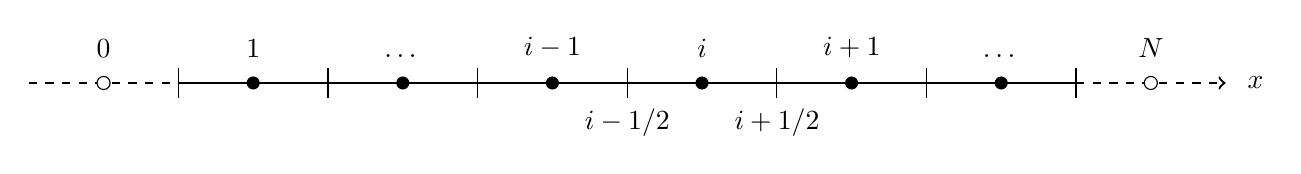
\begin{tikzpicture}[scale=1.9]
	\draw [thick] (0,0) -- (6,0);
	\draw [dashed,thick] (-1,0) -- (0,0);
	\draw [->,dashed,thick] (6,0) -- (7,0);

	\node at (7.2,0) {$x$};

    \def\celllabel[#1](#2){
        \node[fill=black,circle, scale=0.0, label={[yshift=2mm]above:$#2$}] at (#1+0.5,0) {};
    }

    \def\cell(#1){
        \node[fill=black,circle, scale=0.5] at (#1+0.5,0) {};
    }

    \def\ghostcell(#1){
        \node[circle, draw=black, fill=white, scale=0.5] at (#1+0.5,0) {};
    }

    \def\face(#1){
        \draw (#1,0.1) -- (#1, -.1); 
    }

    \def\facelabel[#1](#2){
        \node[scale=0.0, label={[yshift=-2mm]below:$#2$}] at (#1,0) {};
    }

    % draw faces
	\foreach \i in {0,1,...,6}{
		\face(\i);	
	}

    % draw face labels
    \facelabel[3](i-1/2);
    \facelabel[4](i+1/2);

    % draw cell centers
    \foreach \i in {0,1,...,5}{
        \cell(\i);
	}

    % draw ghost cells
    \ghostcell(-1);
    \ghostcell(6);

    % draw cell labels
    \celllabel[-1](0);
    \celllabel[0](1);
    \celllabel[1]($\ldots$);
    \celllabel[2](i-1);
    \celllabel[3](i);
    \celllabel[4](i+1);
    \celllabel[5]($\ldots$);
    \celllabel[6](N);
\end{tikzpicture}
\label{fig:1d_domain}
\caption{Quasi one dimensional domain discretization for the cell-centered finite volume method.}
\end{figure}

\begin{equation}
\mathbf{R}(\Delta t^n, U^n) = \mathbf{S}_i^n - \frac{1}{\Delta x_i} \left( \mathbf{F}^{n}_{i+1/2} - \mathbf{F}^{n}_{i-1/2} \right) 
\label{eq:q1d_euler_res}
\end{equation}

The system of equations is then integrated in time using a 4th-order Runge-Kutta scheme, whit timestep $\Delta t$ determined by imposiv a CFL number

\begin{align}
    k_1 &= \mathbf{R}(t^n, U^n)  \\
    k_2 &= \mathbf{R}(t^n + \frac{\Delta t^n}{2}, U^n +  \Delta t^n \frac{k_1}{2}) \\
    k_3 &= \mathbf{R}(t^n + \frac{\Delta t^n}{2}, U^n +  \Delta t^n \frac{k_2}{2}) \\
    k_4 &= \mathbf{R}(t^n + \Delta t^n, U^n + \Delta t^n k_3) \\
    \mathbf{U}^{n+1} &= \mathbf{U}^n + \frac{1}{6}(k_1 + 2k_2 + 2k_3 + k_4)
\end{align}

The quasi one-dimensional numerical method used in this work is an in-house cfd solver for the compressible Euler equations \eqref{eq:q1d_euler}. Altough the method can capture compressible effects and shock formation, the shock is sharper than the viscous one. The method is also unable to predict the diamond structure of oblique shocks. The method also does not take into account any prescribed tempeture in the wall. 

\subsubsection{Numerical Verification and Validation}

To evaluate the validity of the method, results from our implementation was compered with numerical results obtained by

NUMERICAL VALIDATAION/VERIFICATION of 

\section{Problem Setup}


The nozzle 
A complete geometric description and experimental data for various operational conditions can be found in \cite{Back1965a}. Figure \ref{fig:geom_params} displays the geometric parameters, and the corresponding values are listed in the table \ref{fig:geom_params}.




\subsubsection{Discretization}
\subsubsection{Numerial Verification and Validation}

\subsection{2D Navier-Stokes Solver}
\label{sec:2d_navier_stokes_solver}

The compressible Navier-Stokes equation \eqref{eq:ns_equations} was solved in 2D.

\begin{equation}
    \mathbf{R(\mathbf{U})} = \frac{\partial \mathbf{U}}{\partial t} + \nabla \cdot \mathbf{F}^c(\mathbf{U}) - \nabla \cdot \mathbf{F}^v(\mathbf{U}, \nabla \mathbf{U}) - \mathbf{S}
    \label{eq:navier-stokes}
\end{equation}


\begin{eqnarray}
   %\symbl{$\partial$}{Partial derivative}
   \mathbf{U} = \begin{bmatrix} \rho \\ \rho \mathbf{v} \\ \rho E \end{bmatrix} 
   & \mathbf{F}^c = \begin{bmatrix} \rho \mathbf{v}  \\ \rho \mathbf{v}\otimes \mathbf{v} + \mathbf{1} p \\ \rho E \mathbf{v} + p \mathbf{v} \end{bmatrix} 
   & \mathbf{F}^v = \begin{bmatrix} \cdot \\ \boldsymbol{\tau} \\ \boldsymbol{\tau} \cdot \mathbf{v} + \kappa \nabla T \end{bmatrix} 
   %& \mathbf{S} = \begin{bmatrix} 0 \\ 0  \\ 0 \end{bmatrix}
   \label{eq:ns_equations}
\end{eqnarray}

, with a viscous stress tensor given by 

\begin{equation}
    \boldsymbol{\tau} = \mu \left( \nabla \mathbf{v} + \nabla \mathbf{v}^T \right) - \mu \frac{2}{3} \mathbf{1} \left( \nabla \cdot \mathbf{v} \right)
    \label{eq:ns_stress_tensor}
\end{equation}

The viscosity is

\begin{equation}
    \mu = \mu_d + \mu_t
    \label{eq:mu}
\end{equation}

and the thermal conductivity

\begin{equation}
    \kappa = \frac{\mu_d + c_p}{Pr_d} + \frac{\mu_t c_p}{Pr_t}
    \label{eq:kappa}
\end{equation}

where $\rho$ is the fluid density, $\mathbf{v} = \left\{ u , v \right\}^T \in \mathbb{R}$ is the flow velocity vector, with $u$ and $v$ being its components. $E$ is the total energy per unit mass, $p$ the static pressure, $\boldsymbol{\tau}$ the viscous stress tensor, $T$ the static temprature, $\kappa$ the thermal conductivity, and $\mu$ the viscosity.

With an assumption of a perfect gas, with constant specific heat ratios $\gamma$, and gas constant $R$, the system can be closed using the relation 
for pressure

\begin{equation}
    p = \rho \left( \gamma - 1 \right) \left[ E - \frac{1}{2} \left( \mathbf{v} \cdot \mathbf{v} \right) \right]
    \label{eq:pressure}
\end{equation}

The temperature $T=p/(\rho R)$.

The SU2 software \cite{Economon2016a} was employed to address the conjugate heat transfer interfaces between the fluid and solid in the nozzle. In the fluid domain, the Reynolds Averaged Navier-Stokes equations were solved using the finite volume method and the SST (Shear Stress Transport) turbulence model. To obtain the steady-state solution, the implicit Euler integration method was utilized in conjunction with time marching. On the other hand, for the solid domain, the energy equation was solved.

A Grid Independence Study using the Grid Convergence Index (GCI) \cite{Roache1994} was performed to assess numerical accuracy. Table 1 lists the three mesh levels used and Table 2 shows the results. Positive p and small GCI values indicate a monotonic and asymptotic convergence, respectively. A GCIasymptotic close to 1 indicates grid-independent solutions, so Medium was chosen for further analysis (shown in Figure 2).


\begin{figure}[h]
  \begin{minipage}{0.45\columnwidth}
  \centering
  \includegraphics[width=\hsize]{Figuras/validation/validation_medium.pdf}
  \caption{}
  \captionof{figure}{Validation using all experimental data of reference \cite{Back1965a} for the nozzle in question.\label{fig:validation_su2}}
  \end{minipage}
  \begin{minipage}{0.55\columnwidth}
  \centering
    \begin{tabular}{lcccc}
    \toprule
    & $ \bar{p} $ & $ N_{cells} $ & $ r $ & $ GCI $ \\ \midrule
    Fine & $9.995\times10^4$ & $6000$ & $1.5$ & $0.17$\% \\ 
    Medium & $9.980\times10^4$ & $2500$  & $1.3$ & $0.41$\% \\ 
    Coarse & $9.950\times10^4$ & $1500$  & -   & -  \\ 
    & $ \bar{p}_{extrapolated} $ & & $ order $ &  $ GCI_{asymp.} $ \\ \cline{2-5}
    &  $1.00\times10^5$  &  & $1.99$  &  $1.002$  \\ [0.5ex] \midrule     
    & $ \bar{T} $ & $ N_{cells} $ & $ r $ & $ GCI $\\ \midrule 
    Fine & $6.909\times10^2$ & $6000$ & $1.5$ & $0.00$\% \\ 
    Medium & $6.910\times10^2$ & $2500$  & $1.3$ & $0.04$\%\\ 
    Coarse & $6.930\times10^2$ & $1500$  & -   & -   \\ 
    & $ \bar{T}_{extrapolated} $ & & $ order $ &  $ GCI_{asymp.} $ \\ \cline{2-5}
    & $6.91\times10^2$  &  &  $8.14$ &  $1.000$   \\
    \bottomrule
    \end{tabular}
    \captionof{table}{Grid convergence study over 3 grids.\label{tab:gci_study}}
  \end{minipage}
\end{figure}

\section{Design of Eperiments}

As the method is data driven, data must be gattered or generated. In this study three distincts datasets was generated using a Latin Hypercube Sampling using 1000 iterations to maximize the minimal \textit{pdist}. The ranges for the independent variables is described in Table \ref{tab:doe_lhs}. The surrogate model should be able to reconstruct any flow field of simulations within the precribed design of experiment space of parameters. The dataset consist onluy of converged simulations, the convergence criteria utilized is the maximum residue of $10^{-8}$ for the mass, momementum and energy equation. The dataset was also split into training, validation and test, using $90$ \% of total data for training, 5 \% for validation and the remaining 5 \% for testing.



\begin{table}[h!]
  \centering
  \begin{tabular}{c c c c c c c c} 
   \hline
            & \multicolumn{4}{c}{Design Parameters}  &  \multicolumn{3}{c}{} \\
            & $p_0$ [MPa] & $T_0$ [K] & $\theta_{div}$ [$^\circ$] & $T_w$ [K] & \multicolumn{3}{c}{Dataset Size} \\
    Dataset & (min,max) & (min,max) & (min,max) & (min,max) & Training & Validation & Test \\
   \hline\hline
   Small & \multirow{3}{*}{$(0.31, 1.73)$} & \multirow{3}{*}{$(294.44, 833.33)$} & \multirow{3}{*}{$(10.00, 20.00)$} & \multirow{3}{*}{$(117.78, 541.67)$} & 162 & 8 & 9 \\ 
   Medium &  &  & & & 421 & 21 &  22\\
   Large &  &  & & & 796 & 40 &  40\\
   \hline
  \end{tabular}
  \caption{Dataset ranges for design variables and final dataset sizes retaining converged simlation.}
  \label{tab:doe_lhs}
\end{table}


Since our method relies entirely on data, where the data comes from doesn't matter—it could be gathered through experiments or artificially created using any numerical method. In this study, we're using synthetic data because it makes it easy and quick to control numerical experiments, especially in terms of the number of experiments and the quality of the data.

Regardless of the situation, the first step is to gather two sets of data: one with low fidelity and the other with high fidelity. The low-fidelity data could be a simulation with a rough grid, shortened dimensions, or other simplifications, and it might only include global scalar variables like geometry parameters and averaged boundary conditions. In the world of fluid dynamics, the high-fidelity dataset usually involves multidimensional simulations, trying to capture as much of the physics as possible.

\begin{table}[h!]
    \centering
    \begin{tabular}{c c c c c} 
     \hline
     \textbf{Input} & \textbf{Dataset Size}  &\textbf{Input Components} &  \textbf{Output}  & \textbf{Output Components}\\ 
     \hline
     \hline
     \multirow{15}{*}{$\begin{bmatrix} p \\ T \\ M \\ A \\ T_{wd} \\ p_0 \\ T_0 \\ T_w \\ \theta_{div} \end{bmatrix}^{}$ } & \multirow{5}{*}{Small}  & \multirow{5}{*}{\{2,7,12,...,162\}} & $\begin{bmatrix} p \end{bmatrix}$    & \multirow{4}{*}{\{2,7,12,...,162\}} \\ 
                            & &                                     & $\begin{bmatrix} T \end{bmatrix}$ & \\ 
                            & &                                     & $\begin{bmatrix} M \end{bmatrix}$        & \\ 
                            & &                                     & $\begin{bmatrix} p & T & M & q \end{bmatrix}$  & \\ \cline{4-5}
                            & &                                     & $\begin{bmatrix} q \end{bmatrix}$   & \{2,7,12,...,98\} \\ \cline{2-5}
                        
      & \multirow{5}{*}{Medium} & \multirow{5}{*}{\{2,7,12,...,418\}} & $\begin{bmatrix} p \end{bmatrix}$    & \multirow{4}{*}{\{2,7,12,...,418\}} \\ 
                            & &                                     & $\begin{bmatrix} T \end{bmatrix}$ & \\ 
                            & &                                     & $\begin{bmatrix} M \end{bmatrix}$       & \\ 
                            & &                                     & $\begin{bmatrix} p & T & M & q \end{bmatrix}$  & \\ \cline{4-5}
                            & &                                     & $\begin{bmatrix} q \end{bmatrix}$   & \{2,7,12,...,98\} \\ \cline{2-5}

     & \multirow{5}{*}{Large} & \multirow{5}{*}{\{2,7,12,...,497\}} & $\begin{bmatrix} p \end{bmatrix}$    & \multirow{4}{*}{\{2,7,12,...,794\}} \\ 
                            & &                                     & $\begin{bmatrix} T \end{bmatrix}$ & \\ 
                            & &                                     & $\begin{bmatrix} M \end{bmatrix}$        & \\ 
                            & &                                     & $\begin{bmatrix} p & T & M & q \end{bmatrix}$ & \\ \cline{4-5}
                            & &                                     & $\begin{bmatrix} q \end{bmatrix}$   & \{2,7,12,...,98\} \\
    \hline
    \end{tabular}
    \caption{Table to test captions and labels.}
    \label{table:1}
\end{table}


\section{Hyperparameter Optimization}

Due to previous results and Hyperparameter optimization of the neural Networks was conducted using a small imput dimension with onlyh 5 latent variables and a fixed high dimension for the output fields (400 principal components)


\subsection{Projection Error Analysis}

It is a commonplace procedure to determine the appropriate number of singular values for truncation by assessing the energy or explained variance of the reconstructed matrix $\mathbf{\tilde{X}}$ following reprojection with a truncated basis. However, our investigations reveal that this method is less effective than evaluating the sensitivity of surrogate model accuracy concerning the number of principal components employed. This is due to the fact that a more accurate basis does not necessarily correspond to a more accurate surrogate. To gauge model sensitivity regarding the number of principal components utilized, a series of numerical studies was undertaken. Kriging served as the surrogate model in these studies, with the objective of identifying the minimal number of principal components required to maintain high accuracy.

The search space for this study is the truncated rank of SVD decomposition for the low and high fidelity simulation datasets. The maximum allowed rank is determined by the full matrix of snapshots rank, and could be bounded by the number of samples or the full dimension of each sample. 


\section{Dimensionality Reduction}

The flow reconstruction technique is specifically devised for addressing fluid flow fields, where the number of degrees of freedom is intricately tied to the elements in a full-order numerical simulation. In 3D flow fields, this association can result in an exceedingly large number of degrees of freedom, often reaching millions or even billions. Even in the context of the simplified 2D numerical simulation presented in this study, the number of degrees of freedom is on the order of $10^4$. This numerical value signifies the variables that the surrogate model must encapsulate. Therefore, any reduction in this count not only reflects a judicious application of compressed data but also yields a more cost-effective model.

In addition to the computational efficiency gained by diminishing the computational burden required for modeling the flow field, the process of dimensionality reduction also enhances the model's fitting capabilities. This is owing to the substantial reduction in the number of coupled linear equations that need to be modeled. In essence, the streamlined approach not only contributes to computational economy but also augments the model's efficacy in representing the underlying fluid dynamics.

To enact data compression, the matrices that compile training snapshots for low-fidelity and high-fidelity simulations, denoted as $\mathbf{X}_{l}$ and $\mathbf{X}_h$ respectively, underwent compression utilizing the truncated Singular Value Decomposition (SVD) technique. In essence, the SVD factorization, expressed in equation \ref{eq:svd}, possesses the capability to precisely represent any matrix $\mathbf{X}$ if the number of elements in the diagonal of the square singular values matrix $\mathbf{\Sigma}$ equals the original rank of the matrix $\mathbf{X}$. 

\begin{equation}
    \mathbf{X} = \mathbf{U}\mathbf{\Sigma}\mathbf{V}^T  
    \label{eq:svd}
\end{equation}

Data compression is then achieved by truncating the number of singular values, retaining only the most significant ones, those with higher absolute values arranged in decreasing order. This process serves to distill essential information from the matrices, offering an effective means of compression while maintaining fidelity to the underlying data structure.
